%xelatex
\documentclass[12pt]{extreport}
%\documentclass[14pt]{extreport}

\usepackage{listings}
%\usepackage{verbatim}
\usepackage[T2A]{fontenc}
\usepackage[english,ukrainian]{babel}
\usepackage{mathspec}
\setallmainfonts{Nimbus Roman}
\usepackage{graphicx}
\usepackage[a4paper,margin=0.5in]{geometry}
\usepackage{tikz}
\usetikzlibrary{calc,positioning,shapes.geometric,shapes.symbols,shapes.misc}
\usepackage{indentfirst}
\usepackage{moreverb}
\usepackage{caption}
\usepackage{subcaption}
\usepackage{subfiles}

\lstset{
  basicstyle=\ttfamily,
  columns=fullflexible,
  breaklines=true,
  postbreak=\raisebox{0ex}[0ex][0ex]{\color{red}$\hookrightarrow$\space}
}

\begin{document}

\subfile{title.tex}

%{\fontsize{18}{20.7}\selectfont \textbf{Лабораторна робота №1}}
%{\fontsize{14}{16.1}\selectfont
\subsubsection*{Мета роботи}
Навчитися використовувати структури та об’єднання у мові С.

\bigskip
\subsubsection*{Завдання № 1}
Скласти програму що дає змогу з використанням структур та об'єднань
реалізувати розв’язок поставленої задачі. Всі вхідні дані беруться з текстового
файлу (створити не менше десяти відповідних записів у файлі). Ввід-вивід даних
та виконання інших окремих логічних дій необхідно реалізувати в окремих
функціях. У головній функції необхідно виконувати лише їх виклик.
Використання глобальних змінних не допускається. Інформація повинна
передаватися у функції лише за допомогою параметрів.

В файлі записана інформація про студентів груп бакалаврату, яка
складається з прізвища, імені, статі і віку. Вивести на друк шифр групи в
якій найбільший \% дівчат.
\bigskip

Схема алгоритму зображена на рис. 1 та 2.

\begin{figure}[h]
	\centering
	\subfile{fch.tex}
	\caption{Схема алгоритму для першого завдання}
\end{figure}

\begin{figure}[h]
	\begin{subfigure}[b]{.3\textwidth}
	\centering
		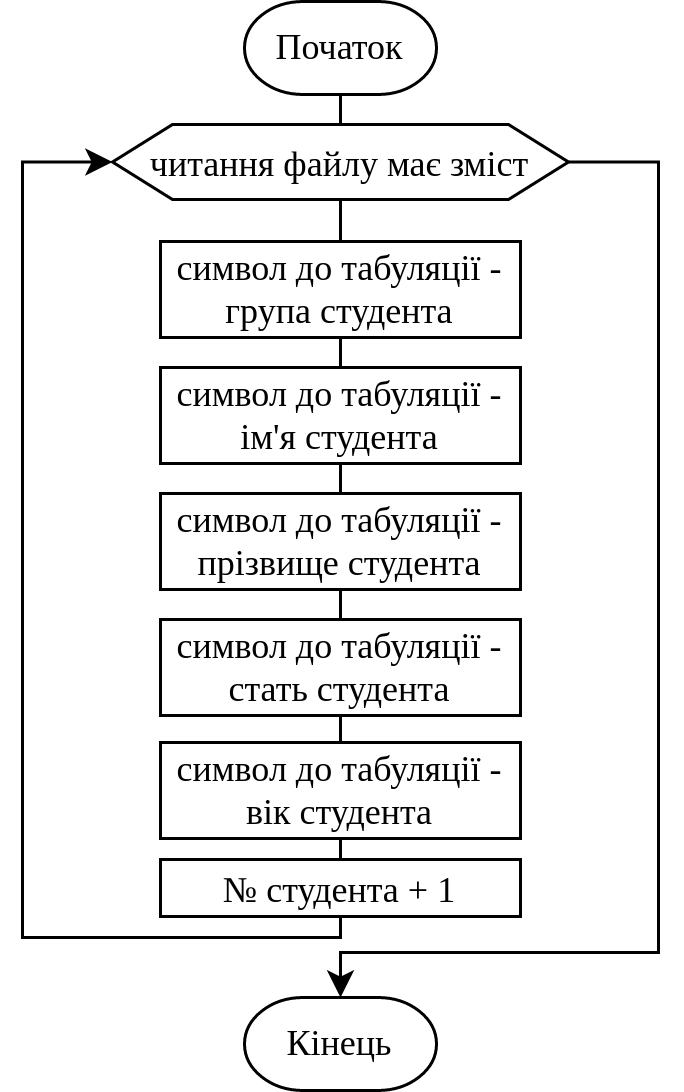
\includegraphics[width=\textwidth]{fch/read.png}
		\caption{функція перетворення тексту на структуру}
	\end{subfigure}
	\hfill
	\begin{subfigure}[b]{.3\textwidth}
	\centering
		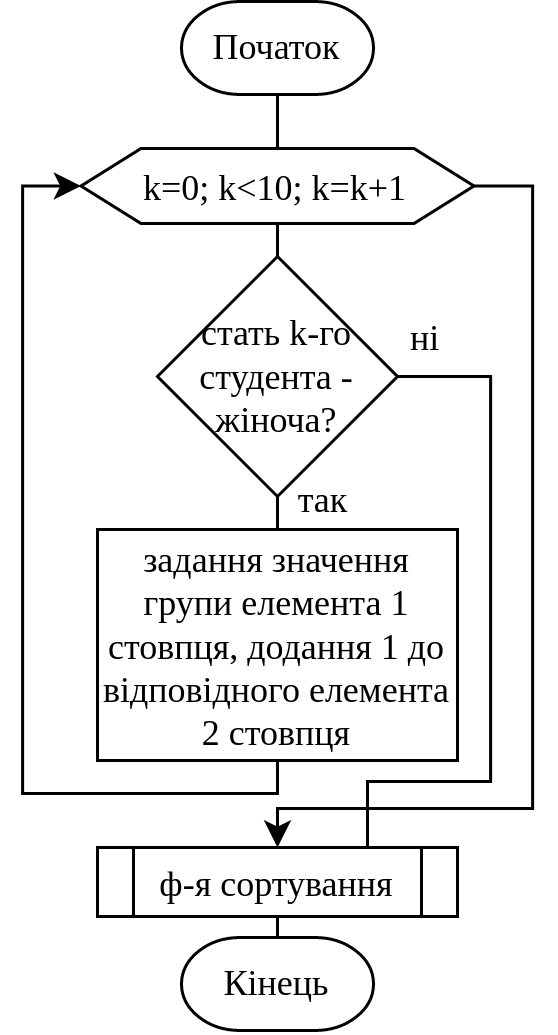
\includegraphics[width=.9\textwidth]{fch/femdetect.png}
		\caption{функція пошуку студентів-дівчат}
	\end{subfigure}
	\hfill
	\begin{subfigure}[b]{.3\textwidth}
	\centering
		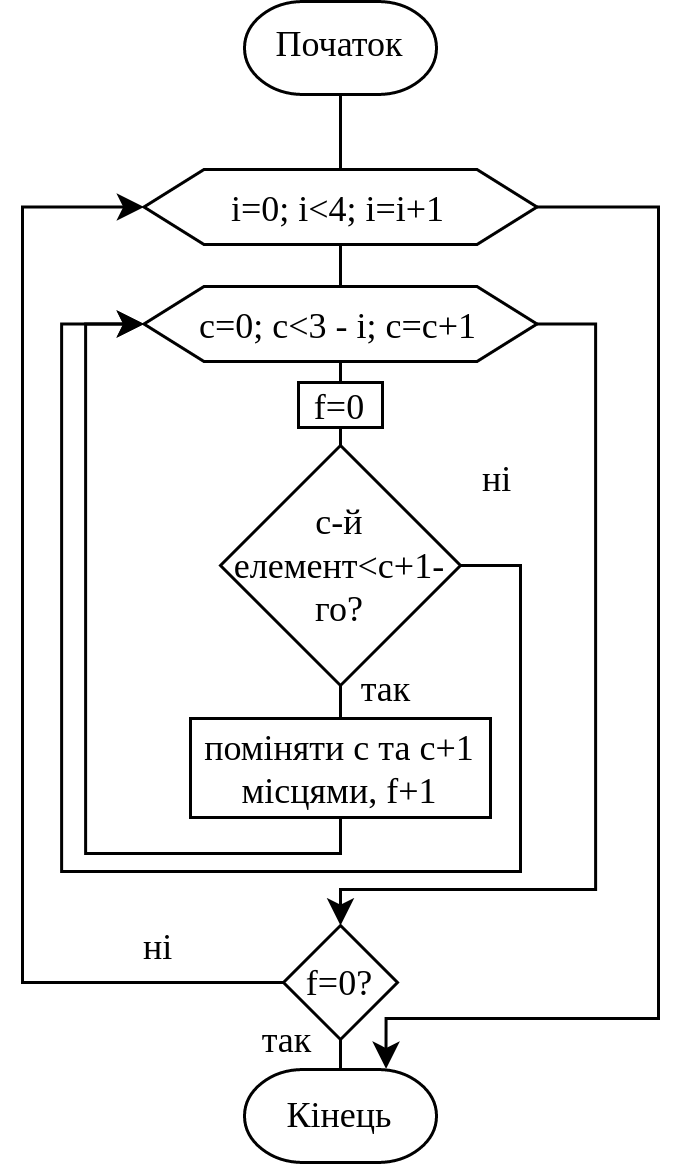
\includegraphics[width=\textwidth]{fch/sort.png}
		\caption{функція сортування}
	\end{subfigure}
	\caption{Схема алгоритму для першого завдання}
	\label{task2}
\end{figure}

\newpage
\subsubsection*{Програмний код до першого завдання}

\begin{lstlisting}[frame=single]
#include <stdio.h>
#include <string.h>
#include <stdlib.h>

struct ug{
	int group;
	char fname[12];
	char lname[12];
	int gen;
	int age;
};

void write(int m[4][2]){
	printf("Group containing the most female undergraduates: %d",m[0][0]);
}

struct ug *readstrct(){
	struct ug d[10];
	FILE *fp;
	char str[121];
	char *item;
	int id=0, k;

	fp=fopen("eqr","r");

	while (fgets(str, 120, fp)){

		item=strtok(str,"\t");
		d[id].group=atoi(item);

		item=strtok(NULL,"\t");
		strcpy(d[id].fname, item);

		item=strtok(NULL,"\t");
		strcpy(d[id].lname, item);

		item=strtok(NULL,"\t");
		d[id].gen=atoi(item);

		item=strtok(NULL,"\n");
		d[id].age=atoi(item);

		id++;
	}
	fclose(fp);

	struct ug *p = d;
	return p;
}

void sort(int m[4][2]){
	for(int i=0; i<4; i++){
		int f=0;
		for(int c=0; c<3-i; c++){
			int c1 = m[c][1], c2 = m[c+1][1];
			if(c1==c2) continue;
				if(m[c][1]<m[c+1][1]){
				int ee=m[c][1];
				m[c][1]=m[c+1][1];
				m[c+1][1]=ee;

				int mee=m[c-1][2];
				m[c-1][2]=m[c][2];
				m[c][2]=mee;

				f++;
			}
			if(f==0) break;
		}
	}

	write(m);
}

int femdetect(struct ug *st){
	int e, m[4][2];
	m[0][0]=0;
	for(int k=0; k<10; k++){
		if(st[k].gen==0){
			e = st[k].group;
			m[e-1][1]+=1;
			m[e-1][0]=e;
		}
	}
	sort(m);
}

int main(){
	struct ug *st = readstrct();
	femdetect(st);

	return 0;
}

\end{lstlisting}

Вивід:

\begin{lstlisting}
Group containing the most female undergraduates: 3
\end{lstlisting}

\subsubsection*{Завдання № 2}
Розробити програму яку забезпечує опрацювання структур даних.
Необхідно забезпечити опрацювання 3-5 полів елементів з використанням
різних простих типів даних (стрічки, символи, числа). Забезпечити виконання
таких операцій:
\begin{itemize}
\item додавання нового елементу;
\item пошук елементу за значенням полів;
\item послідовний перегляд елементів;
\item модифікація значень полів елемену;
\item видалення елементу;
\item сортування за значеннями полів.
\end{itemize}

Результати всіх операцій повинні зберігатись у файлі (створити не менше
десяти відповідних записів у файлі). Елемент: Фрукт (назва, країна-постачальник, ціна).

\bigskip
Схема програми зображена на рис. 3-7.

\subsubsection*{Програмний код до другого завдання}

\begin{lstlisting}[frame=single]
#include <stdio.h>
#include <stdlib.h>
#include <string.h>
struct fruits
{
	int id;
	char name[20];
	char country[20];
	int p1;
};
int getnum()//scan number of fruits
{
	int i;
	FILE *fp=fopen("in.txt","r");
	fscanf(fp,"%d",&i);
	fclose(fp);
	return i;
}
void change_num(int i)//change number of fruits
{
	FILE *fp=fopen("in.txt","w");
	fprintf(fp,"%d",i);
	fclose(fp);
}
struct fruits *read_struct(struct fruits *c)//read arr of structures from file
{
	FILE *fptr = fopen("bin.bin","rb");
	fread(c,sizeof(c[0])*getnum(), 1, fptr);
	fclose(fptr);
	return c;
};
void change_struct(struct fruits *c)//write struct to file
{
	FILE *fptr = fopen("bin.bin","wb");
	fwrite(c,sizeof(c[0])*getnum(), 1, fptr);
	fclose(fptr);
};
void print(struct fruits *c)
{
	int i=getnum();
	//print structure
	for (int j=0;j<i;j++)
		printf("%d)ID=%d\tName=%s\tcountry=%s\tprice=%d\n",j+1, c[j].id,c[j].name,c[j].country,c[j].p1);
}
void add(struct fruits *c)
{
	int i=getnum();
	printf("%d\n",i);
	//adding new structure
	printf("Enter id:");		scanf("%d",  &c[i].id);
	printf("Enter name: ");		scanf("%s", c[i].name);
	printf("Enter country:");	scanf("%s", c[i].country);
	printf("Enter price: ");	scanf("%d", &c[i].p1);
	change_num(++i);

	change_struct(c);
}
void del(struct fruits *c){
	int i=getnum();
	// choosing element
	int a;
	printf("Enter id:");
	scanf("%d", &a);
	for(int j=0;j<i;j++)
	{
		if(c[j].id==a)
		{
			//printf("fruit found\n");
			for(int l=0;l<i-j;l++)
			{
				c[j+l]=c[j+l+1];
			}
			i--;
			change_num(i);
			printf("item deleted\n");
			break;
		}
	}
	change_struct(c);
}
void sort(struct fruits *c, int n)
{
	printf("i - sort by id p - sort by price\n");
	char a[5];
	scanf("%s",&a);
	if(*a=='i' || *a=='p'){
		for(int i=0;i<n;++i){
			int f=0;
			for(int j = 0;j < n-i-1; ++j){
				int dif, c1, c2;
				if(*a=='i')
					c1 = c[j].id, c2 = c[j+1].id;
				if(*a=='p')
					c1 = c[j].p1, c2 = c[j+1].p1;
				if(c1==c2)continue;
				dif = c1 - c2;
				if(dif > 0){
					 struct fruits p = c[j];
					 c[j] = c[j + 1];
					 c[j + 1] = p;
					 f++;
				}
			}
			if(f==0)break;
		}
	}
	change_struct(c);
	print(c);
}
void find(struct fruits *c, int n)
{
	char country_to_find[20];
	printf("Enter country:");
	scanf("%s",country_to_find);
	for(int i=0;i<n;i++)
	{
		int flag=0;
		for(int j=0;j<strlen(c[i].country);j++)
			if(c[i].country[j] == country_to_find[j])
				flag++;

		if(flag==strlen(c[i].country)){
			printf("ID= %d\tName=%s\tcountry=%s\tprice=%d\n", c[i].id,c[i].name,c[i].country,c[i].p1);
			break;
		}
	}

}
void change(struct fruits *c, int n)
{
	printf("i - change id n - change name");
	char a[5];
	int d;//id you are going to find
	int newid;
	char fn[20];//finding name
	char newname[20];
	scanf("%s",a);
	switch ( *a ){
	case 'i':
		scanf("%d",&d);
		for(int i=0;i<n;i++){
			if(c[i].id == d){
				printf("Your id matches name %s\nEnter new id:",c[i].name);
				scanf("%d", &newid);
				c[i].id=newid;
			}
		}
	break;
	case 'n':
		scanf("%s",fn);
		for(int i=0;i<n;i++){
			int flag=0;
			for(int j=0;j<strlen(c[i].name);j++)
				if(c[i].name[j] == fn[j])
					flag++;

			if(flag==strlen(c[i].name)){
				printf("Your name matches id %d\nEnter new name:",c[i].id);
				scanf("%s", newname);
				strcpy(c[i].name,newname);
			}
		}
	}
	change_struct(c);
}
int main()
{
	int i=getnum();
	struct fruits c[i+10];
	read_struct(c);
	char q[5];
	printf("a-append\tc-change\tf-find\tl-list\ts-sort\td-delete\tq-quit\n");
	scanf("%s",q);
	switch ( q[0] ){
		case 'l':print(c); break;
		case 'a':add(c);break;
		case 'd':del(c);break;
		case 's':sort(c,i);break;
		case 'f':find(c,i);break;
		case 'c':change(c,i);break;
		case 'q':return 0;
	}
	main();
}
\end{lstlisting}

Вивід:

\begin{lstlisting}
a-append        c-change        f-find  l-list  s-sort  d-delete       q-quit
a
1
Enter id:3
Enter price: 14
a-append        c-change        f-find  l-list  s-sort  d-delete       q-quit
l
1)ID=1  Name=pear       country=Ukraine price=41
2)ID=3  Name=pomegranate        country=Greece  price=14
a-append        c-change        f-find  l-list  s-sort  d-delete       q-quit
c
i - change id n - change namen
pear
Your name matches id 1
Enter new name:apple
a-append        c-change        f-find  l-list  s-sort  d-delete       q-quit
l
1)ID=1  Name=apple      country=Ukraine price=41
2)ID=3  Name=pomegranate        country=Greece  price=14
a-append        c-change        f-find  l-list  s-sort  d-delete       q-quit
a
2
Enter id:2
Enter name: cherry
Enter country:France
Enter price: 31
a-append        c-change        f-find  l-list  s-sort  d-delete
a-append        c-change        f-find  l-list  s-sort  d-delete       q-quit
s
i - sort by id p - sort by price
i
1)ID=1  Name=apple      country=Ukraine price=41
2)ID=2  Name=cherry     country=France  price=31
3)ID=3  Name=pomegranate        country=Greece  price=14
a-append        c-change        f-find  l-list  s-sort  d-delete       q-quit
d
Enter id:1
item deleted
a-append        c-change        f-find  l-list  s-sort  d-delete       q-quit
l
1)ID=2  Name=cherry     country=France  price=31
2)ID=3  Name=pomegranate        country=Greece  price=14
a-append        c-change        f-find  l-list  s-sort  d-delete       q-quit
q
\end{lstlisting}

\newpage
\begin{figure}[h]
	\centering
	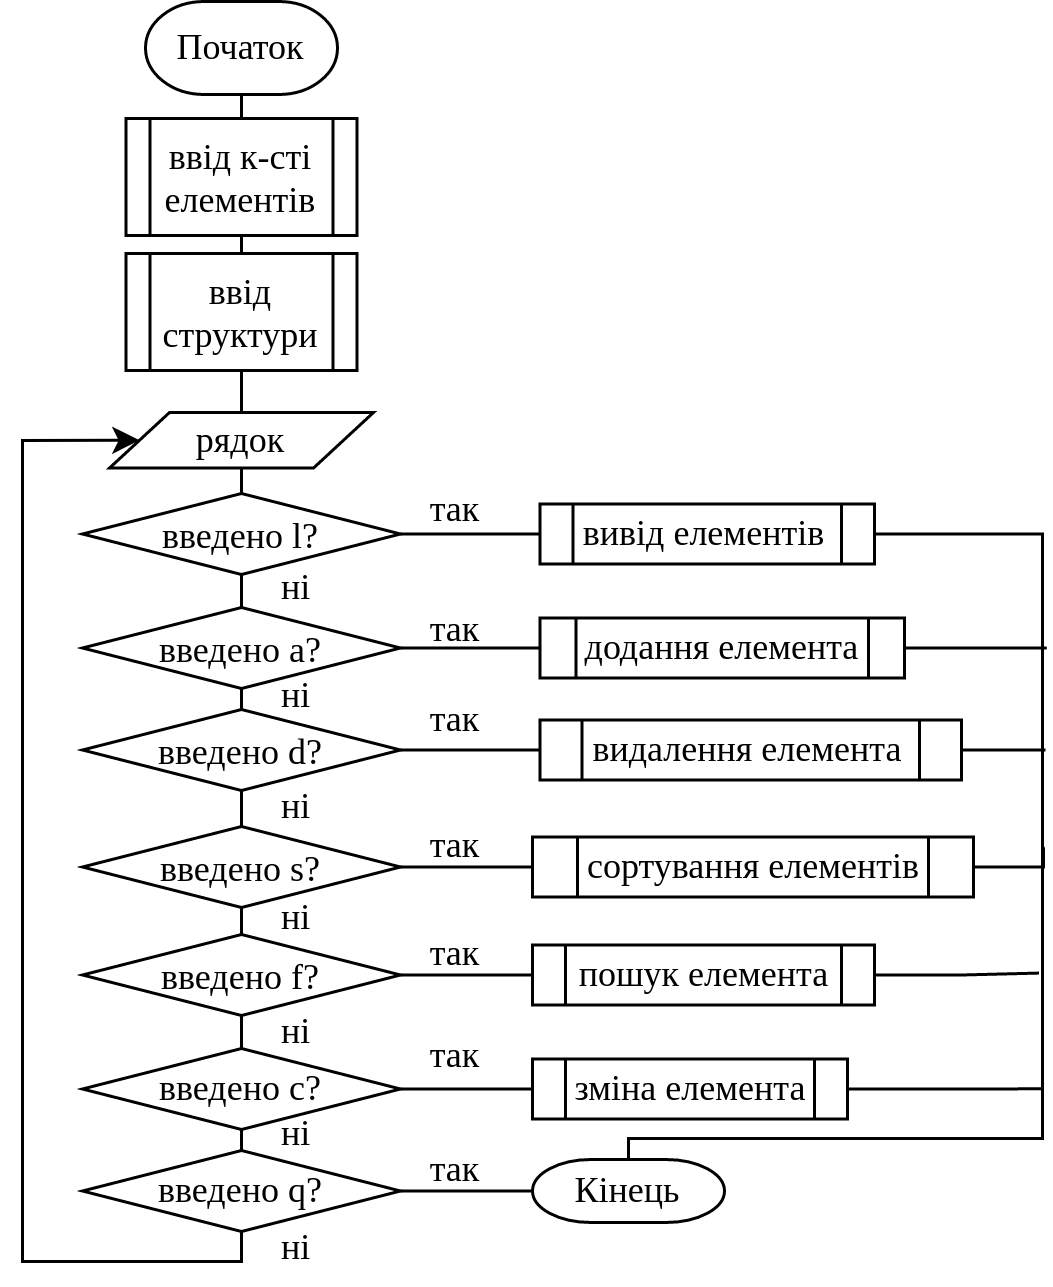
\includegraphics[width=.6\textwidth]{fch2/main.png}
	\caption{Схема головної функції для другого завдання}
	\label{task2}
\end{figure}

\begin{figure}[h]
	\begin{subfigure}[b]{.19\textwidth}
	\centering
		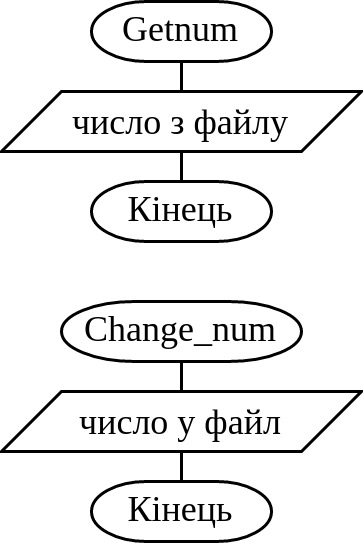
\includegraphics[width=\textwidth]{fch2/getnum.png}
		\caption{Функції читання та запису к-сті фр.}
	\end{subfigure}
	\hfill
	\begin{subfigure}[b]{.24\textwidth}
	\centering
		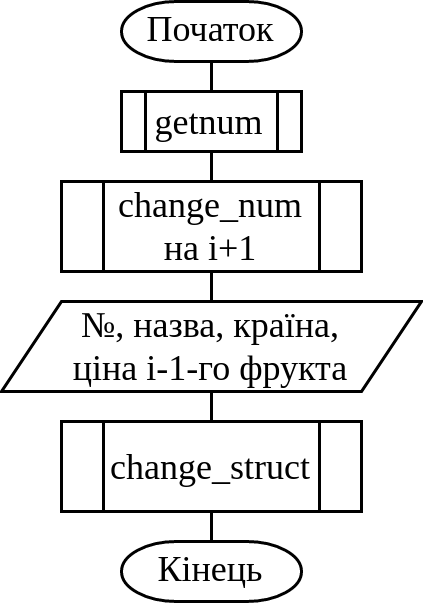
\includegraphics[width=\textwidth]{fch2/add.png}
		\caption{функція додання фрукта}
	\end{subfigure}
	\hfill
	\begin{subfigure}[b]{.28\textwidth}
	\centering
		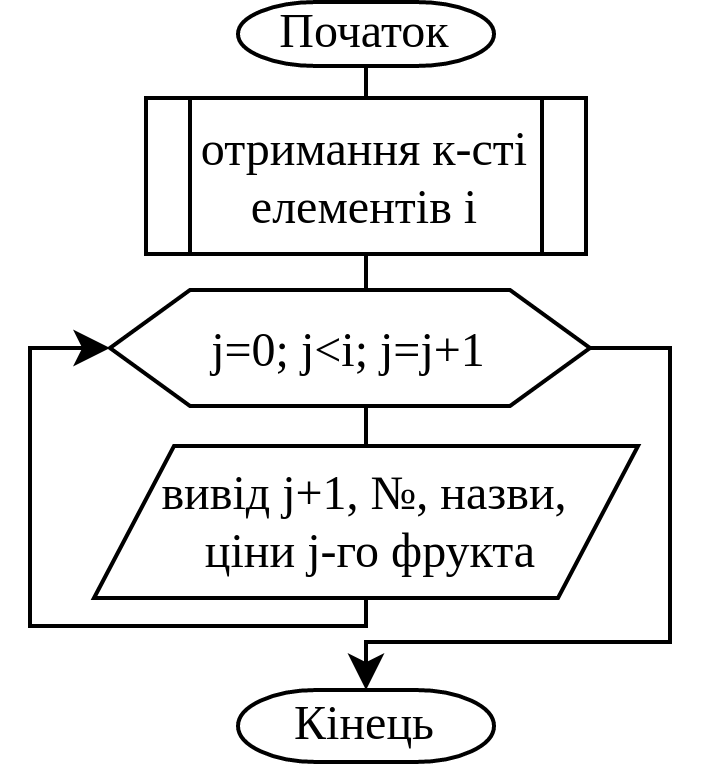
\includegraphics[width=\textwidth]{fch2/print.png}
		\caption{функція виводу структур на друк}
	\end{subfigure}
	\hfill
	\begin{subfigure}[b]{.23\textwidth}
	\centering
		
\includegraphics[width=\textwidth]{fch2/read_struct.png}

		\medskip
		
\includegraphics[width=\textwidth]{fch2/rstruct.png}
		\caption{функції вводу та виводу структур}
	\end{subfigure}
	\caption{}
\end{figure}

\begin{figure}[h]
	\centering
	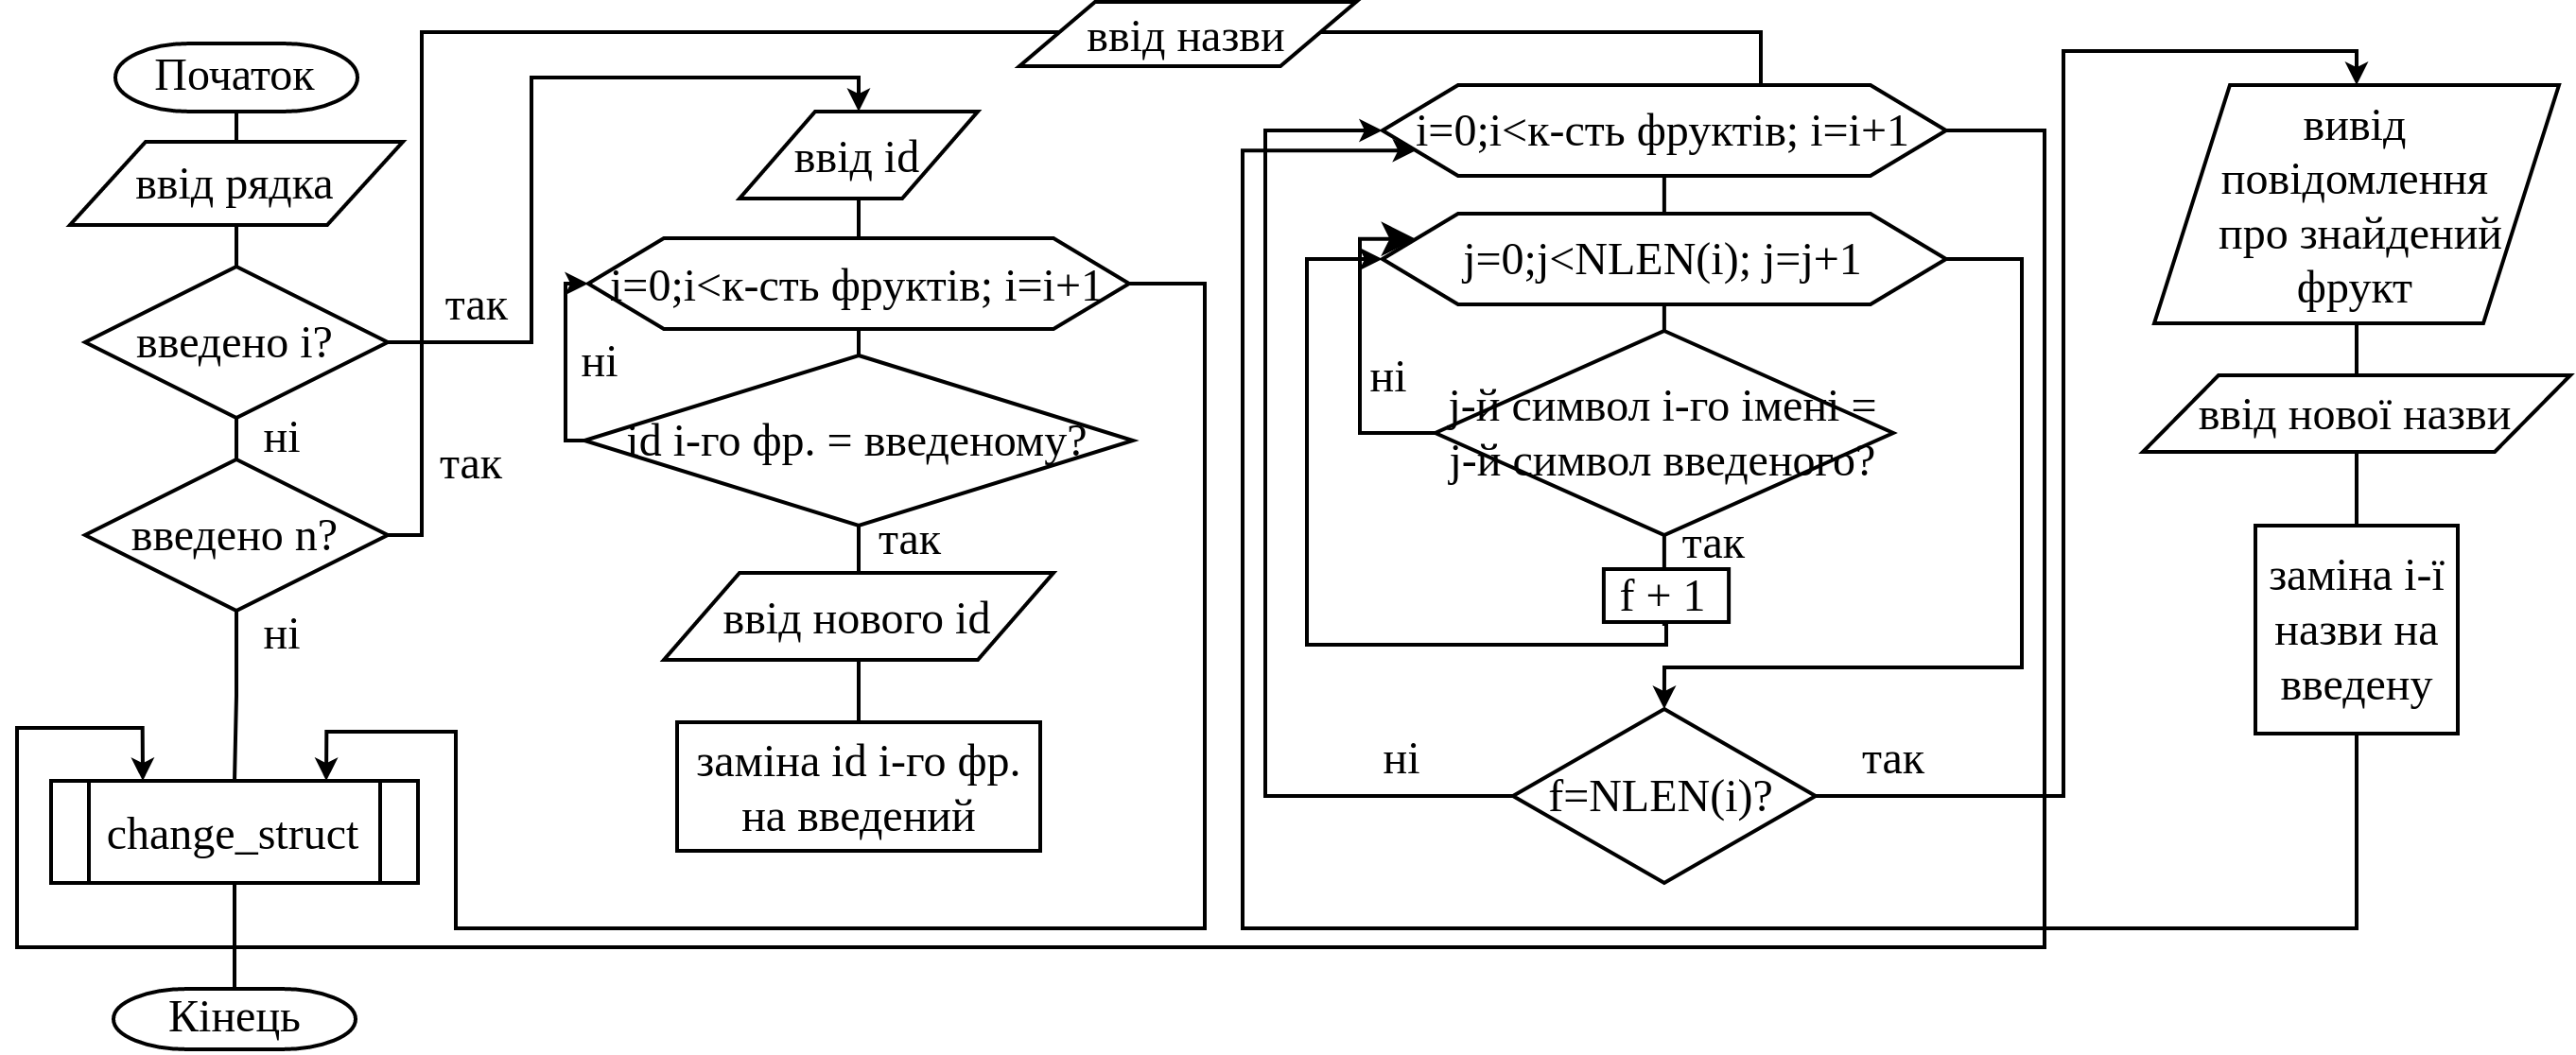
\includegraphics[width=\textwidth]{fch2/change.png}
	\caption{Схема функції для внесення змін у назву та id фрукта. NLEN~--- довжина назви фрукта}
	\label{task2}
\end{figure}

\begin{figure}[h]
	\centering
	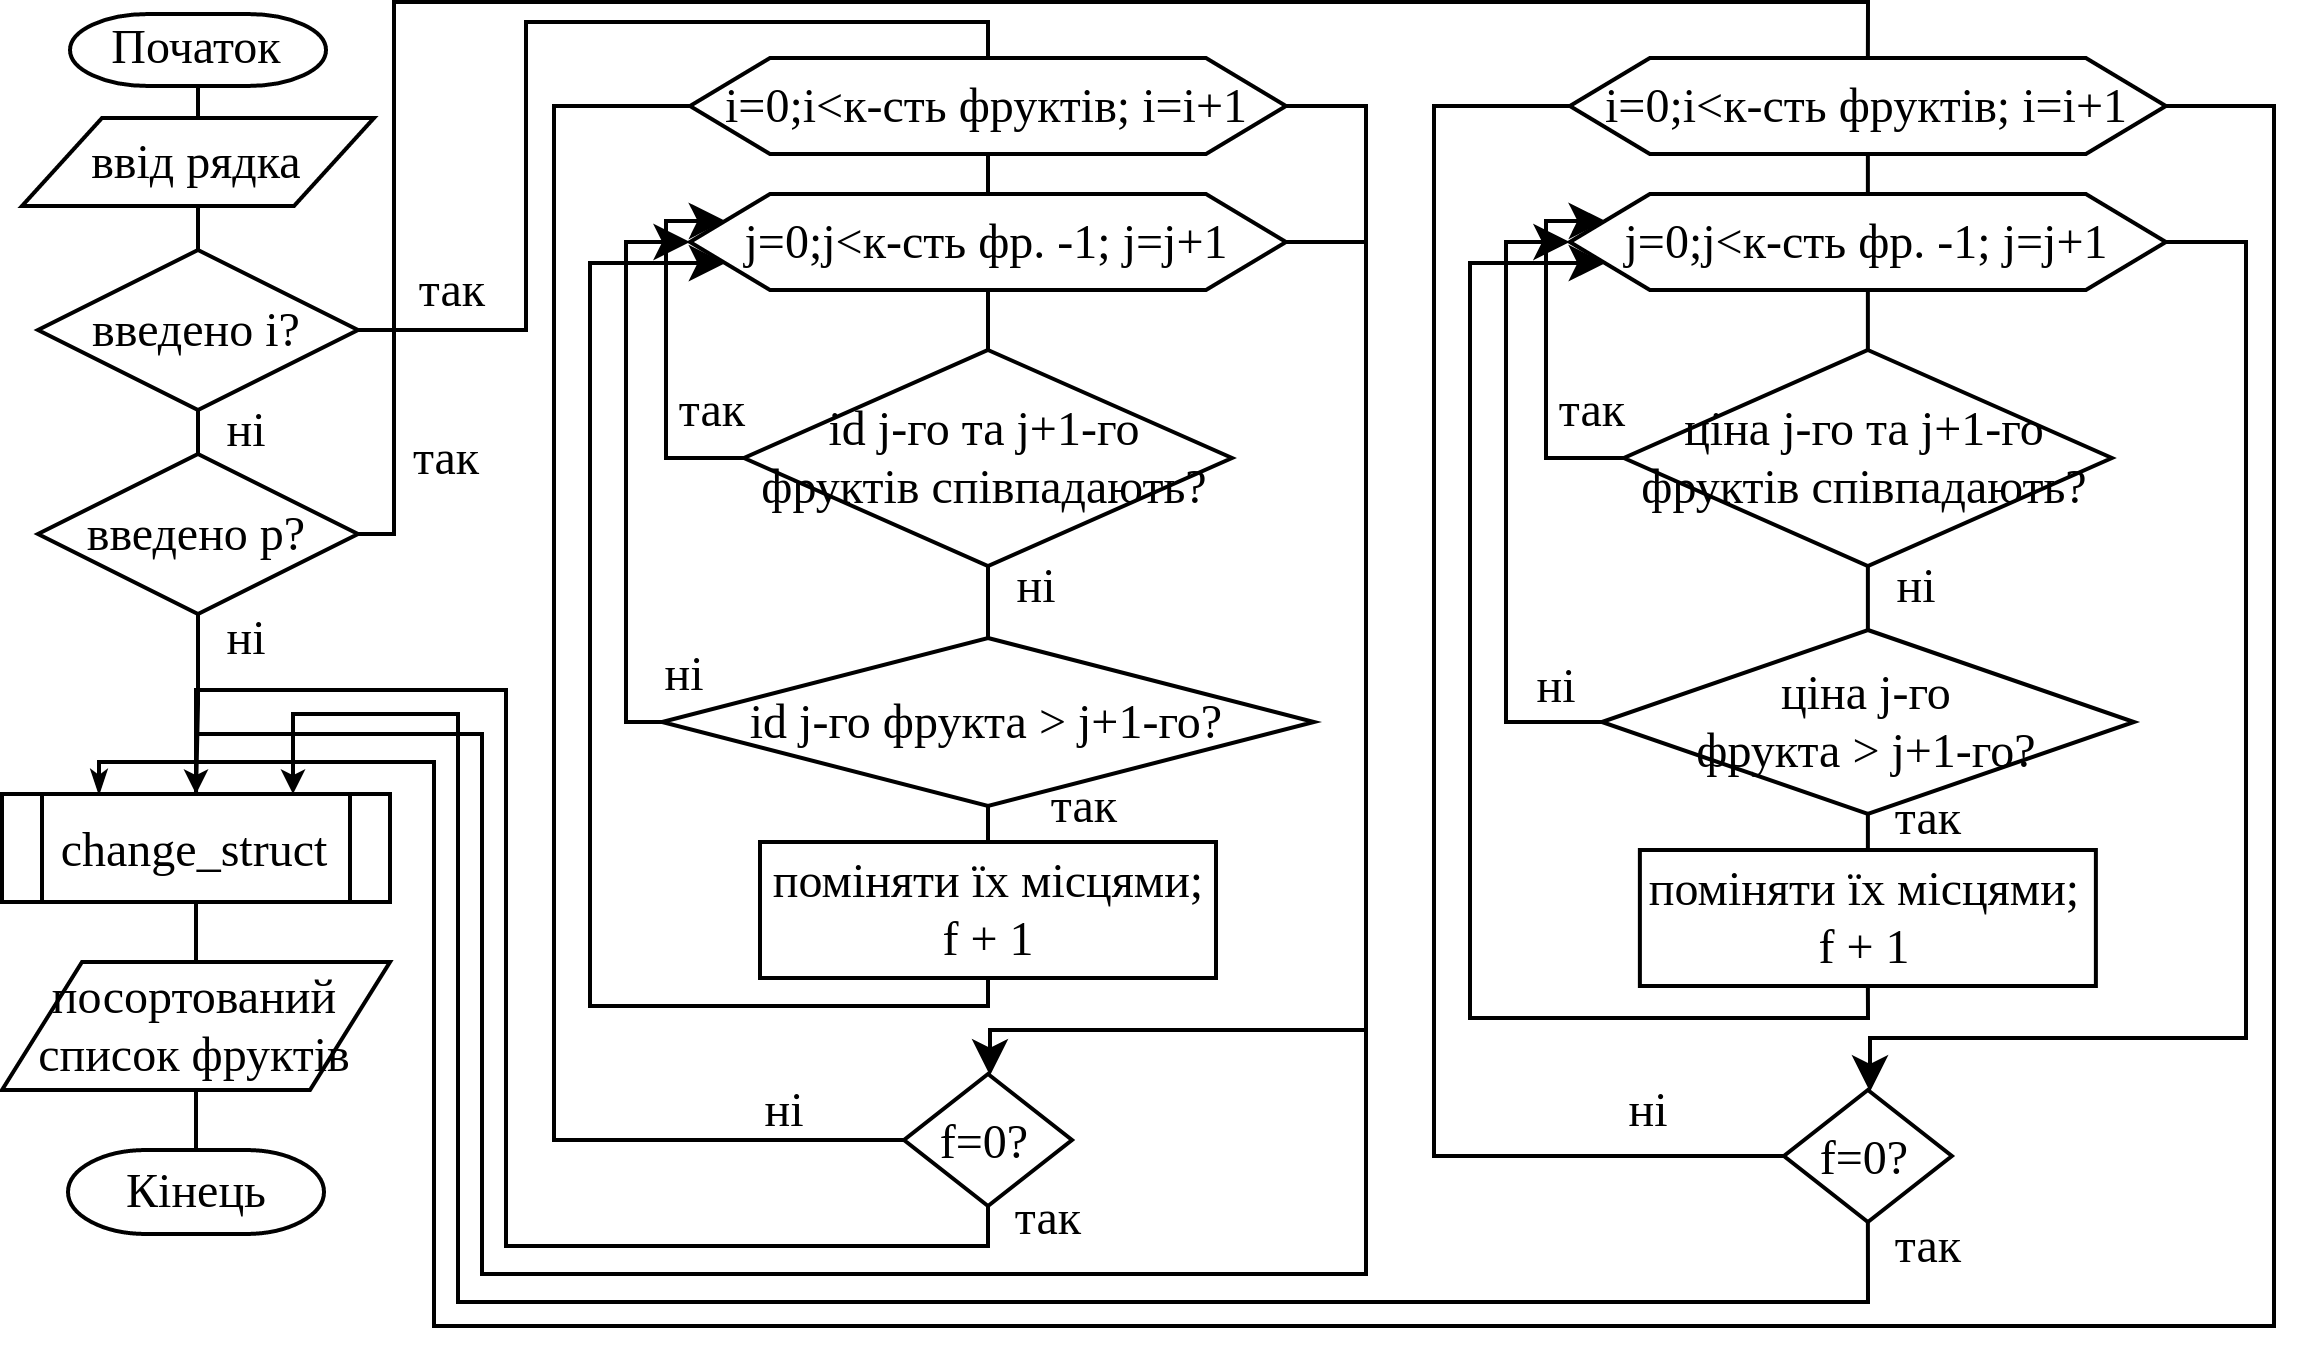
\includegraphics[width=.8\textwidth]{fch2/sort.png}
	\caption{Схема функції сортування структур}
	\label{task2}
\end{figure}

\begin{figure}[h]
	\begin{subfigure}[b]{.5\textwidth}
	\centering
		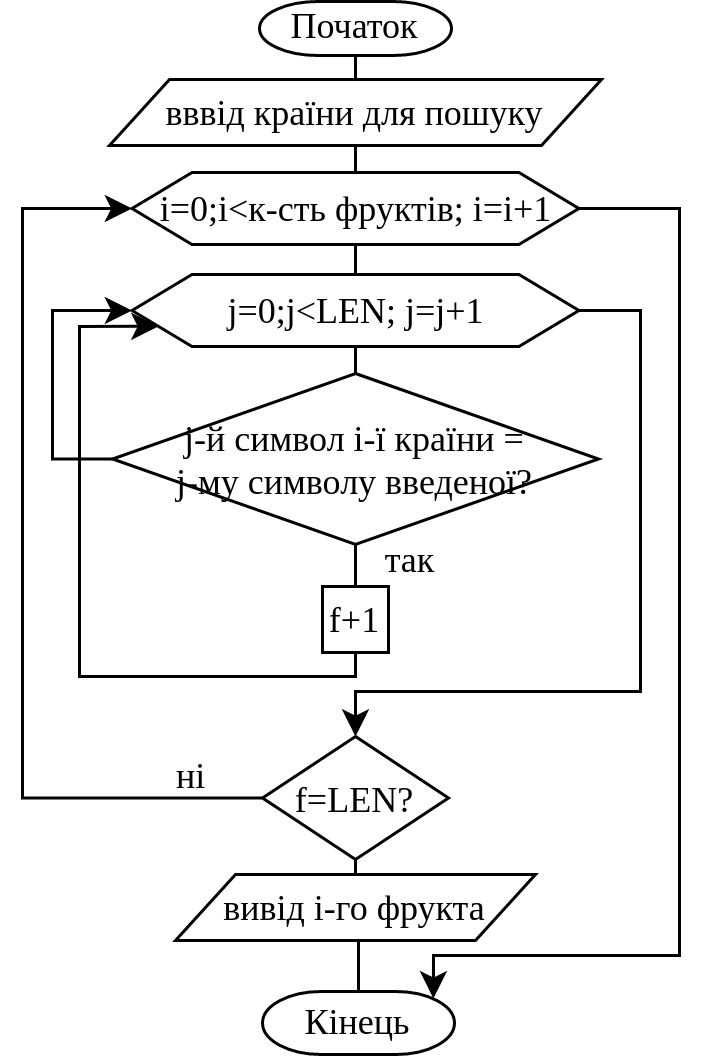
\includegraphics[width=.7\textwidth]{fch2/find.png}
		\caption{функція пошуку структури. LEN~--- к-сть фруктів}
	\end{subfigure}
	\hfill
	\begin{subfigure}[b]{.5\textwidth}
	\centering
		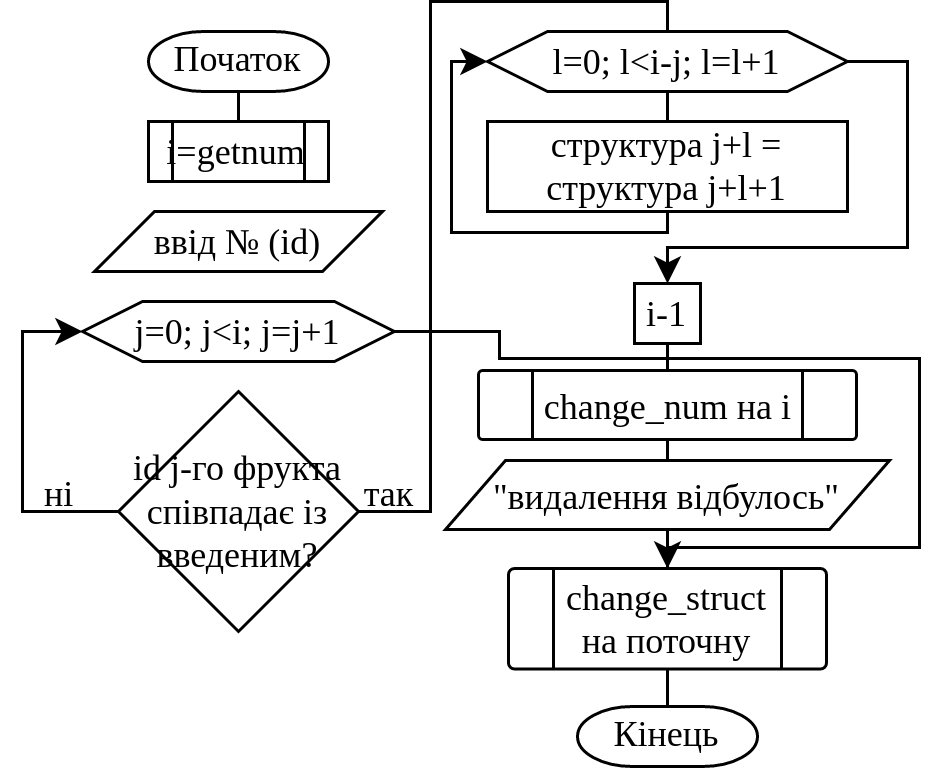
\includegraphics[width=\textwidth]{fch2/del.png}
		\caption{функція видалення структури}
	\end{subfigure}
	\caption{}
\end{figure}


\subsubsection*{Висновок:}
Виконуючи цю лабораторну роботу, я засвоїв роботу зі структурами
в мові C та закріпив уміння, здобуті у процесі виконання попередніх
робіт.

\end{document}
